%%%%%%%%%%%%%%%%%%%%%%%%%%%%%%%%%%%%%%%%%
% Beamer Presentation
% LaTeX Template
% Version 1.0 (10/11/12)
%
% This template has been downloaded from:
% http://www.LaTeXTemplates.com


%----------------------------------------------------------------------------------------
%	PACKAGES AND THEMES
%----------------------------------------------------------------------------------------

\documentclass{beamer}

\mode<presentation> {


\usetheme{Madrid}
\usecolortheme{whale}


\graphicspath{{images/}}

%\setbeamertemplate{footline} % To remove the footer line in all slides uncomment this line
%\setbeamertemplate{footline}[page number] % To replace the footer line in all slides with a simple slide count uncomment this line

\setbeamertemplate{footline}[text line]{
  \parbox{\linewidth}{\vspace*{8pt}, 
\includegraphics[scale=0.1]{logo.pdf}\hfill\hfill\insertpagenumber\vskip4pt}}

\setbeamerfont{footline}{size=\fontsize{7}{7}\selectfont}

\setbeamertemplate{navigation symbols}{} % To remove the navigation symbols from the bottom of all slides uncomment this line
}
\usepackage[utf8]{inputenc}
\usepackage{graphicx} % Allows including images
\usepackage{booktabs} % Allows the use of \toprule, \midrule and \bottomrule in tables
\usepackage{ulem}
\usepackage{color}
\usepackage{amsmath}
\usepackage{array}
\usepackage{multirow}
\usepackage{changepage}
\usepackage{colortbl}
\usepackage{hyperref}
\usepackage{framed}

\usepackage{tcolorbox}

\definecolor{mycolor}{RGB}{255,255,255}

\tcbset{colframe=white,colback=white,nobeforeafter}

\tcbset{
mytext/.style={
  top=0pt,bottom=0pt,left=0pt,right=0pt,colback=gray!10,colframe=structure}
}


\graphicspath{{images/}}

%----------------------------------------------------------------------------------------
%	TITLE PAGE
%----------------------------------------------------------------------------------------

\title{Is pre-registration of studies a bad idea \newline or a very bad idea?} 
\author{Shravan Vasishth (with Daniela Mertzen)} 
\institute[Universität Potsdam] 
{
\medskip
%\textit{mertzen@uni-potsdam.de} 
}
\date{\today} 


\begin{document}

\begin{frame}
\titlepage 
\end{frame}


%----------------------------------------------------------------------------------------
%	PRESENTATION SLIDES
%----------------------------------------------------------------------------------------


\begin{frame}

\begin{center}
\begin{Large}
\textsc{What is a pre-registration?}
\end{Large}
\end{center}

\end{frame}

%------------------------------------------------

\begin{frame}
\frametitle{What is a Pre-Registration?}

\begin{itemize}
\item Specification of \textbf{study hypotheses}, \textbf{design} and \textbf{planned data analysis} strategy before data collection begins. 
\item  Time-stamped on OSF or aspredicted.org, or accepted for publication via a Registered Report.
\end{itemize}


\end{frame}


%------------------------------------------------


\begin{frame}

\begin{center}
\begin{Large}
\textsc{Why is it important to pre-define the analysis plan?}
\end{Large}
\end{center}

\end{frame}

%------------------------------------------------

\begin{frame}
\frametitle{Researcher degrees of freedom make any outcome possible}

\begin{center}
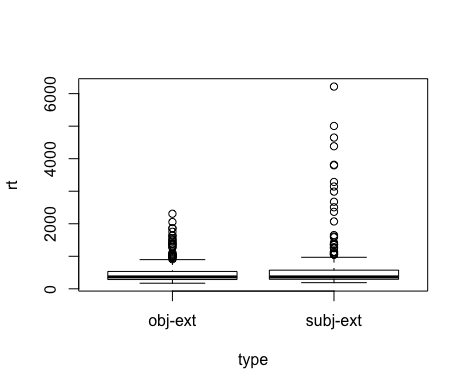
\includegraphics[scale=0.5]{gibsonwudistrn.png}
\end{center}



\end{frame}

\begin{frame}
\frametitle{Researcher degrees of freedom make any outcome possible}
\framesubtitle{Goal: show significant effect}

By subject t-test: t(36) = -2.63, p-value = 0.013 

By item t-test: t(14) = -2.15, p-value = 0.04956


[This was the published result.]
\end{frame}

\begin{frame}[fragile]\frametitle{Researcher degrees of freedom make any outcome possible}
\framesubtitle{Goal: show no significant difference}

\textbf{Take log transform}:

By subject t-test: t(36) = -1.6549, p-value = 0.12

By item t-test: t(14) = -1.62, p-value = 0.13 

\medskip

\textbf{Or fit a linear mixed model on raw RTs}:

\begin{verbatim}
Formula: rt ~ so + (1 + so | subj) + (1 + so | item)
Fixed effects:
            Estimate Std. Error t value
(Intercept)   547.33      53.21  10.287
so             59.85      33.74   1.774
\end{verbatim}
\end{frame}


\begin{frame}[fragile]\frametitle{Researcher degrees of freedom make any outcome possible}
\framesubtitle{Even the meaning of ``statistically significant'' is fluid}

From a JML paper (Dillon et al., 2013):

 ``For total times this analysis \textbf{revealed a three-way interaction} that was significant by participants and marginal by items (F1(1, 39) = 8.0, p $<$ .01; F2(1,47) = 4.0, p $<$ .055; \textbf{minF0 (1, 81) = 2.66, p = .11}). This interaction did not reach significance in either’ first-pass or probability of regression measures.''

\medskip

\textbf{In fact, the interaction is not significant (look at the minF).}

\textbf{Summary}: Interaction in total time, first-pass reading time, first-pass regression not significant
\end{frame}


\begin{frame}[fragile]\frametitle{Researcher degrees of freedom make any outcome possible}
\framesubtitle{Even the meaning of ``statistically significant'' is fluid}

\begin{center}
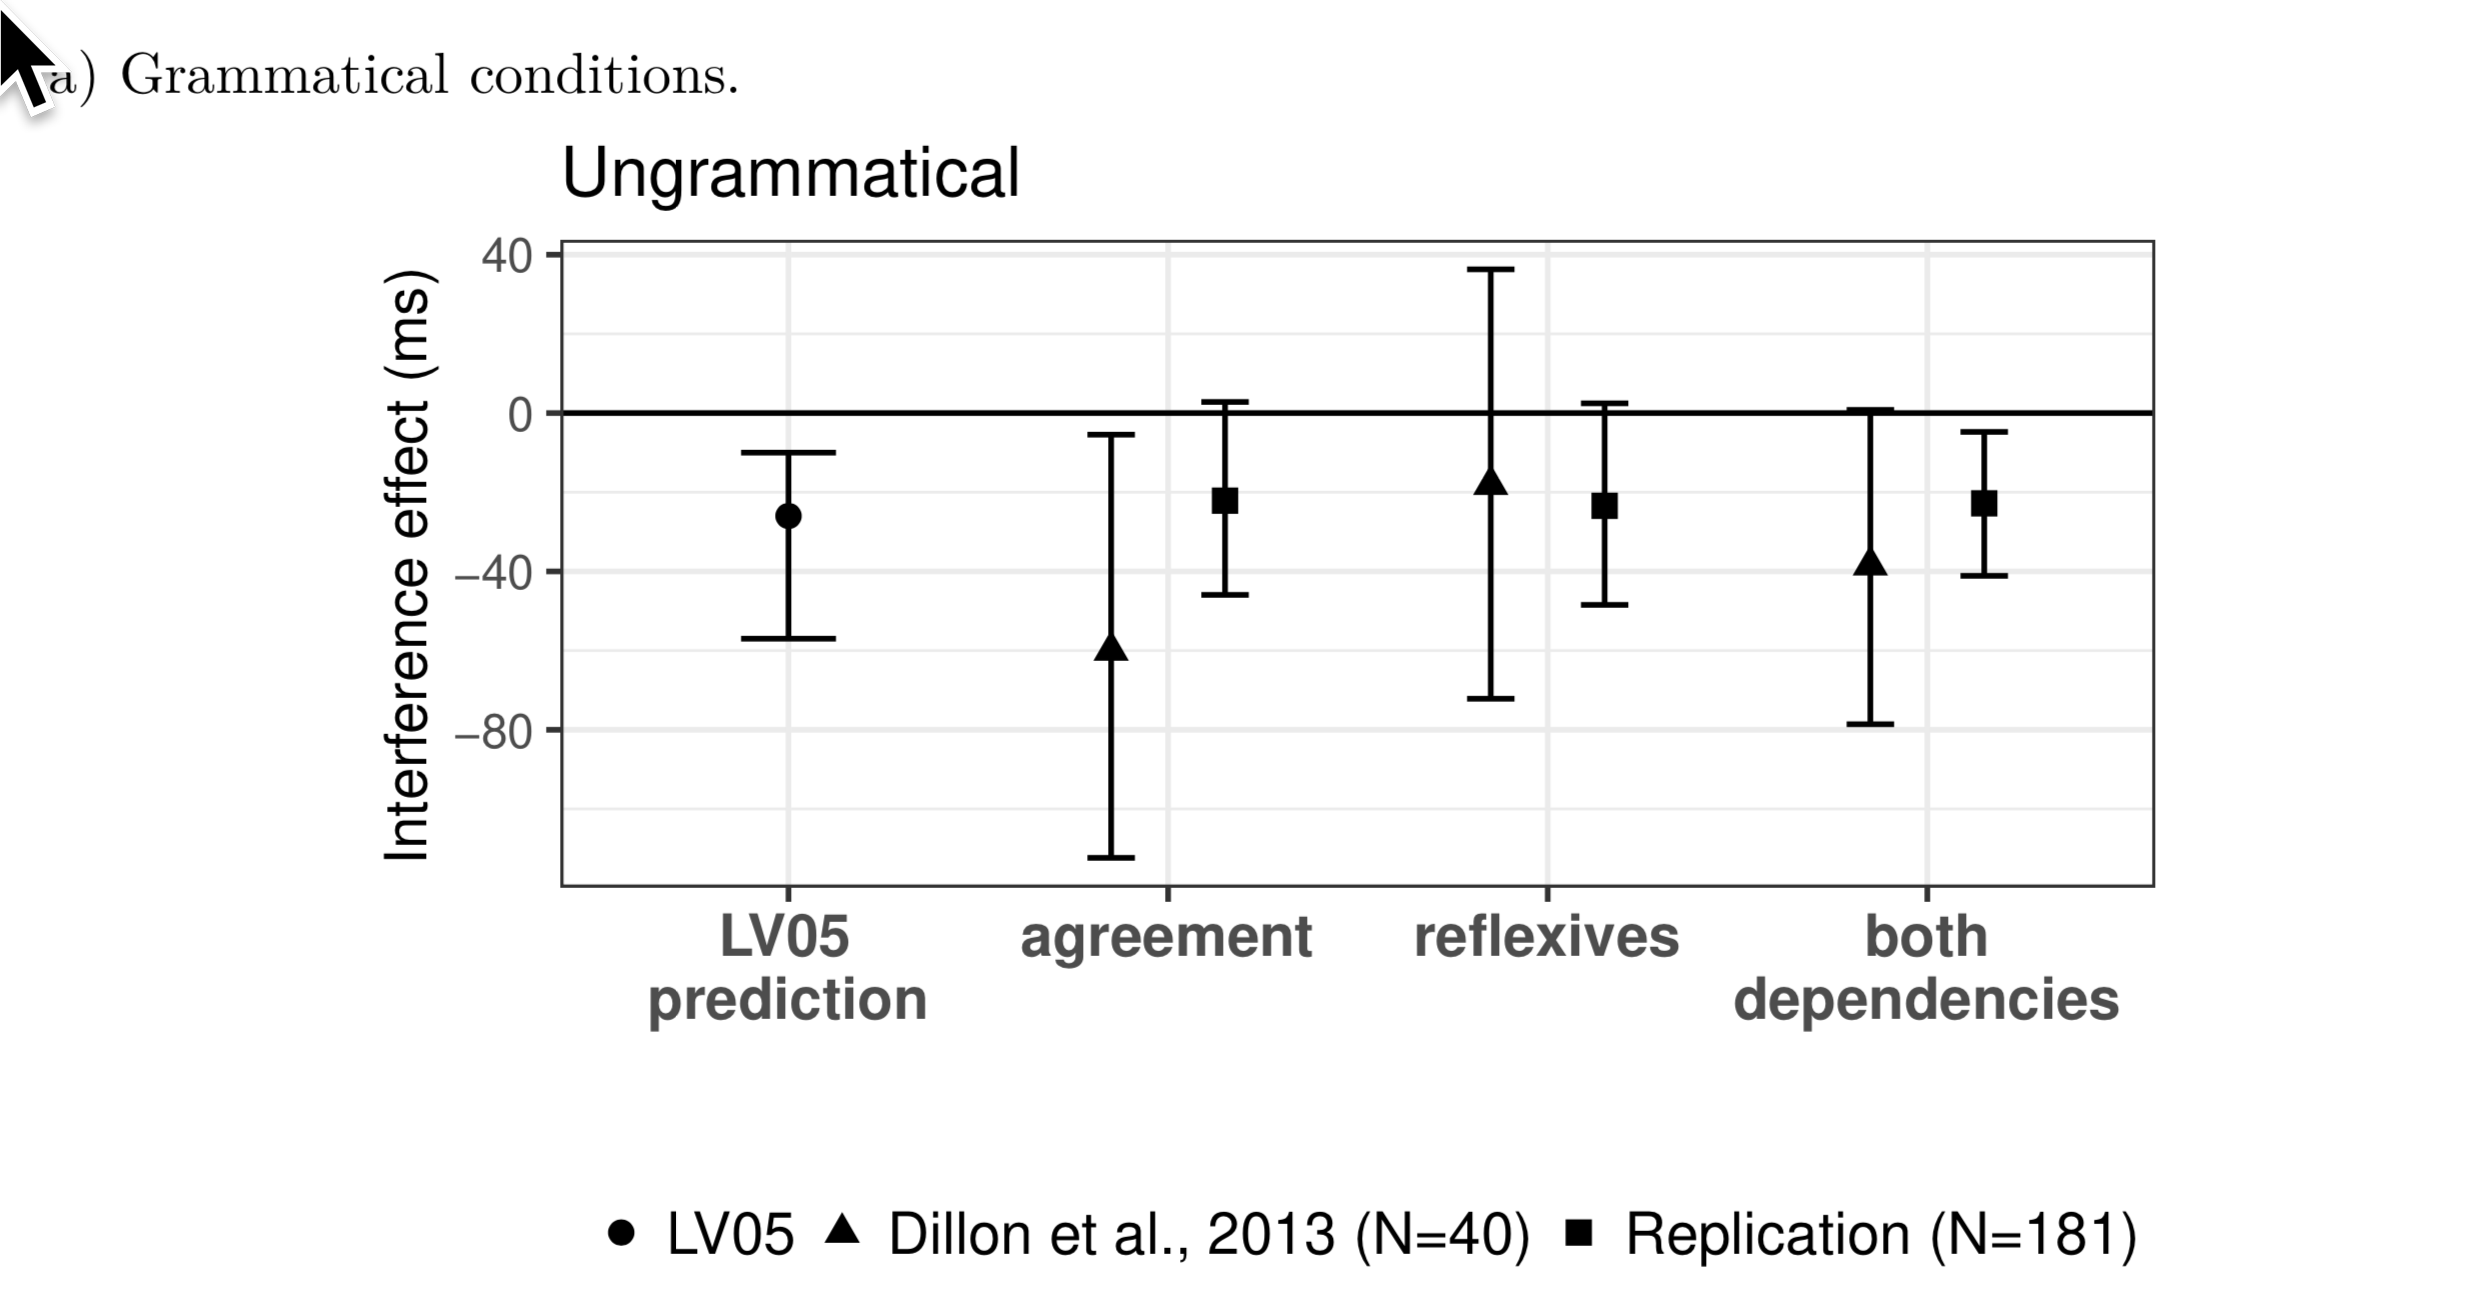
\includegraphics[scale=0.25]{dillonrepTFT.png}
\end{center}


\end{frame}


\begin{frame}[fragile]\frametitle{Researcher degrees of freedom make any outcome possible}
\framesubtitle{Change the dependent measure when the original measure doesn't work out}

In our replication attempt, 
we see the same pattern in \textbf{first-pass regressions} that the original Dillon et al 2013 study found in \textbf{total time}:

\begin{itemize}
\item
agreement: -0.06 [-0.09,-0.02] 
\item 
reflexives: -0.01 [-0.04, 0.03] 
\end{itemize}

\textbf{Question}: Could one now argue that this effect in \textbf{first-pass regressions} confirm the original interaction claimed for \textbf{total time}? Recall that the original study found no effect in first-pass regressions.

\end{frame}

\begin{frame}
\frametitle{Researcher degrees of freedom make any outcome possible}
\framesubtitle{p-hacking and outlier ``management''} 

\begin{center}
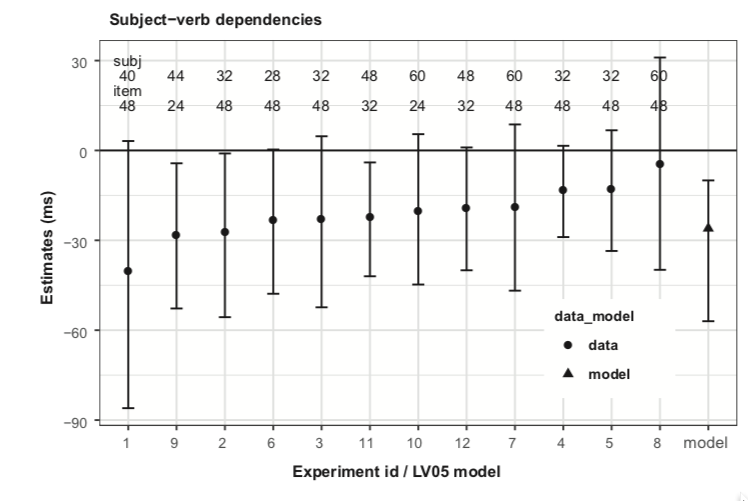
\includegraphics[scale=0.35]{subjverbdeps.png}
\end{center}

\end{frame}

\begin{frame}
\frametitle{Researcher degrees of freedom make any outcome possible}
\framesubtitle{HARKing}

\begin{itemize}
\item Hypothesizing After Results are Known.
\item Researcher knowingly or unknowingly presents an unexpected result as one that has been predicted all along. 
\item Produces clean, confirmatory papers that journals prefer while maintaining illusion that research is hypothesis-driven. 
\end{itemize}


\begin{center}

\includegraphics[scale=0.15]{logacevvasishth.png}
\end{center}

\end{frame}



\section{Replication failures}

\begin{frame}
\frametitle{One consequence of Researcher Degrees of Freedom: The replication crisis}

`Replication crisis' (Open Science Collaboration, 2012) in psychological research: Many results from the literature cannot be reproduced.\\[45pt]

\begin{small}
De Groot (1956/2014) The meaning of “significance” for different types of research.' %[translated and annotated by Eric-Jan Wagenmakers, Denny Borsboom, Josine Verhagen, Rogier Kievit, Marjan Bakker, Angelique Cramer, Dora Matzke, Don Mellenbergh, and Han L. J. van der Maas], In Acta Psychologica, Volume 148, 2014, Pages 188-194, ISSN 0001-6918, https://doi.org/10.1016/j.actpsy.2014.02.001.
\end{small}

\end{frame}

%------------------------------------------------

\begin{frame}
\frametitle{Failures to replicate in psycholinguistics}
\framesubtitle{Nieuwland review of early prediction effects}

\begin{center}
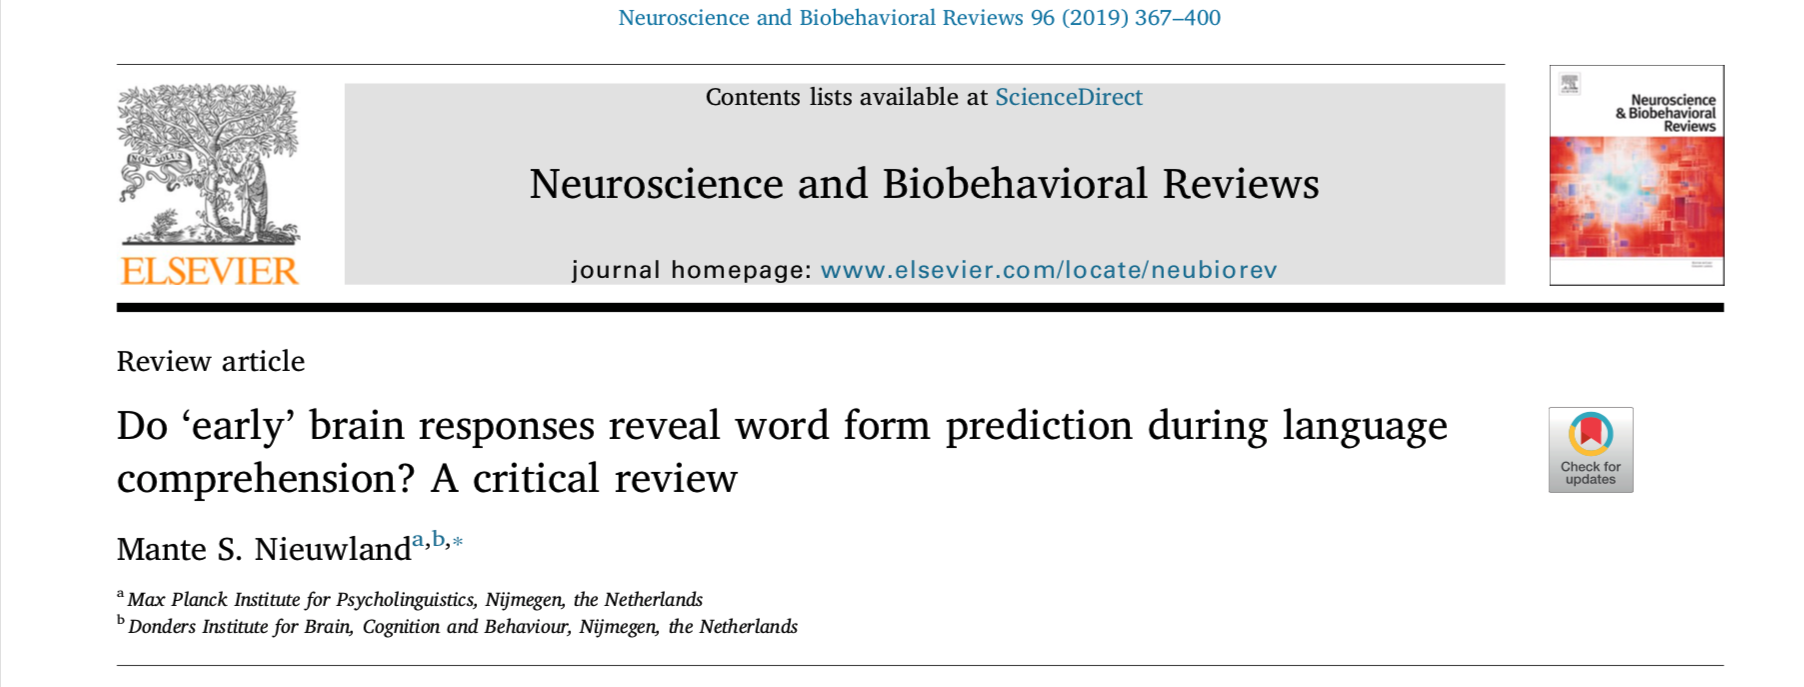
\includegraphics[scale=0.2]{nieuwland2019.png}
\end{center}


\end{frame}


\begin{frame}
\frametitle{Failures to replicate in psycholinguistics}
\framesubtitle{Vasishth et al, replication failure of Levy and Keller, 2013}

\begin{center}

\includegraphics[scale=0.4]{vasishth2018.png}
\end{center}

\end{frame}



%------------------------------------------------

%------------------------------------------------


%------------------------------------------------

\begin{frame}
\frametitle{Big effects get published, but are overestimates}
\framesubtitle{Gelman and Carlin, 2014, J\"ager et al., 2017, Vasishth et al., 2018}

\begin{center}
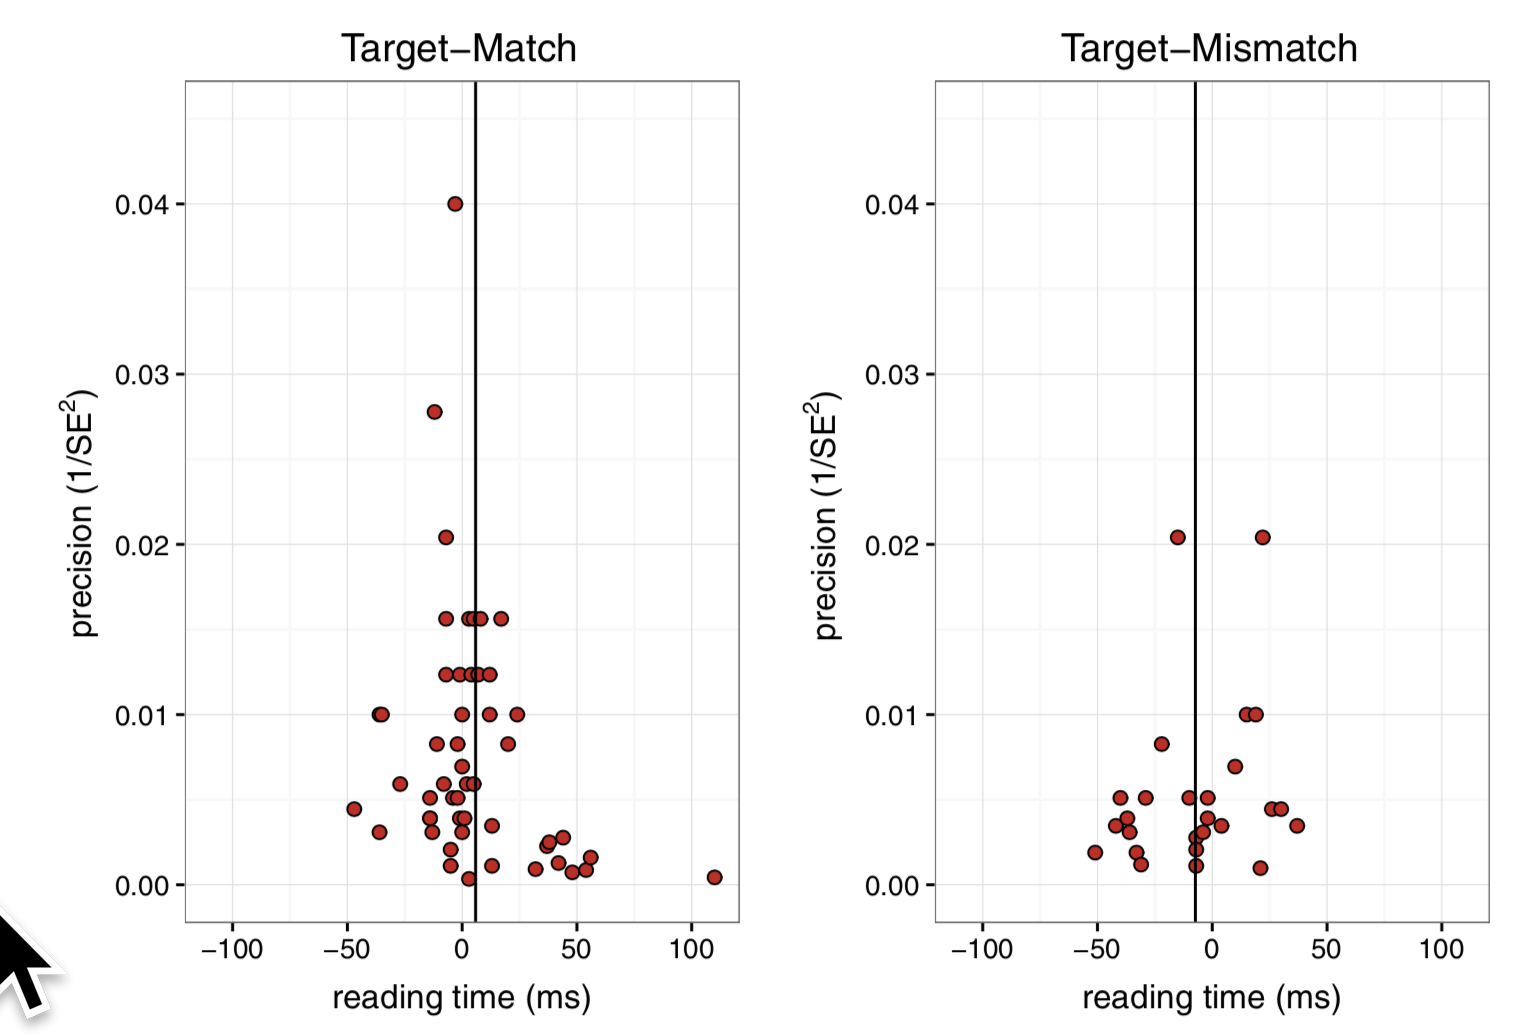
\includegraphics[scale=0.35]{pubbias.png}
\end{center}



\end{frame}
%------------------------------------------------



%------------------------------------------------

\begin{frame}
\frametitle{A solution: Registered reports}

\begin{itemize}
\item \textbf{Registered reports force journal editors to make a decision to publish before results exist.} \\ \pause
$\rightarrow$ Whether these are positive or negative, novel or familiar is irrelevant.
 \pause
\item Exploratory analyses are encouraged, but these will be clearly distinguishable from the confirmatory analysis. 
\end{itemize}

\end{frame}

\begin{frame}
\frametitle{A solution: Registered reports}

\begin{center}
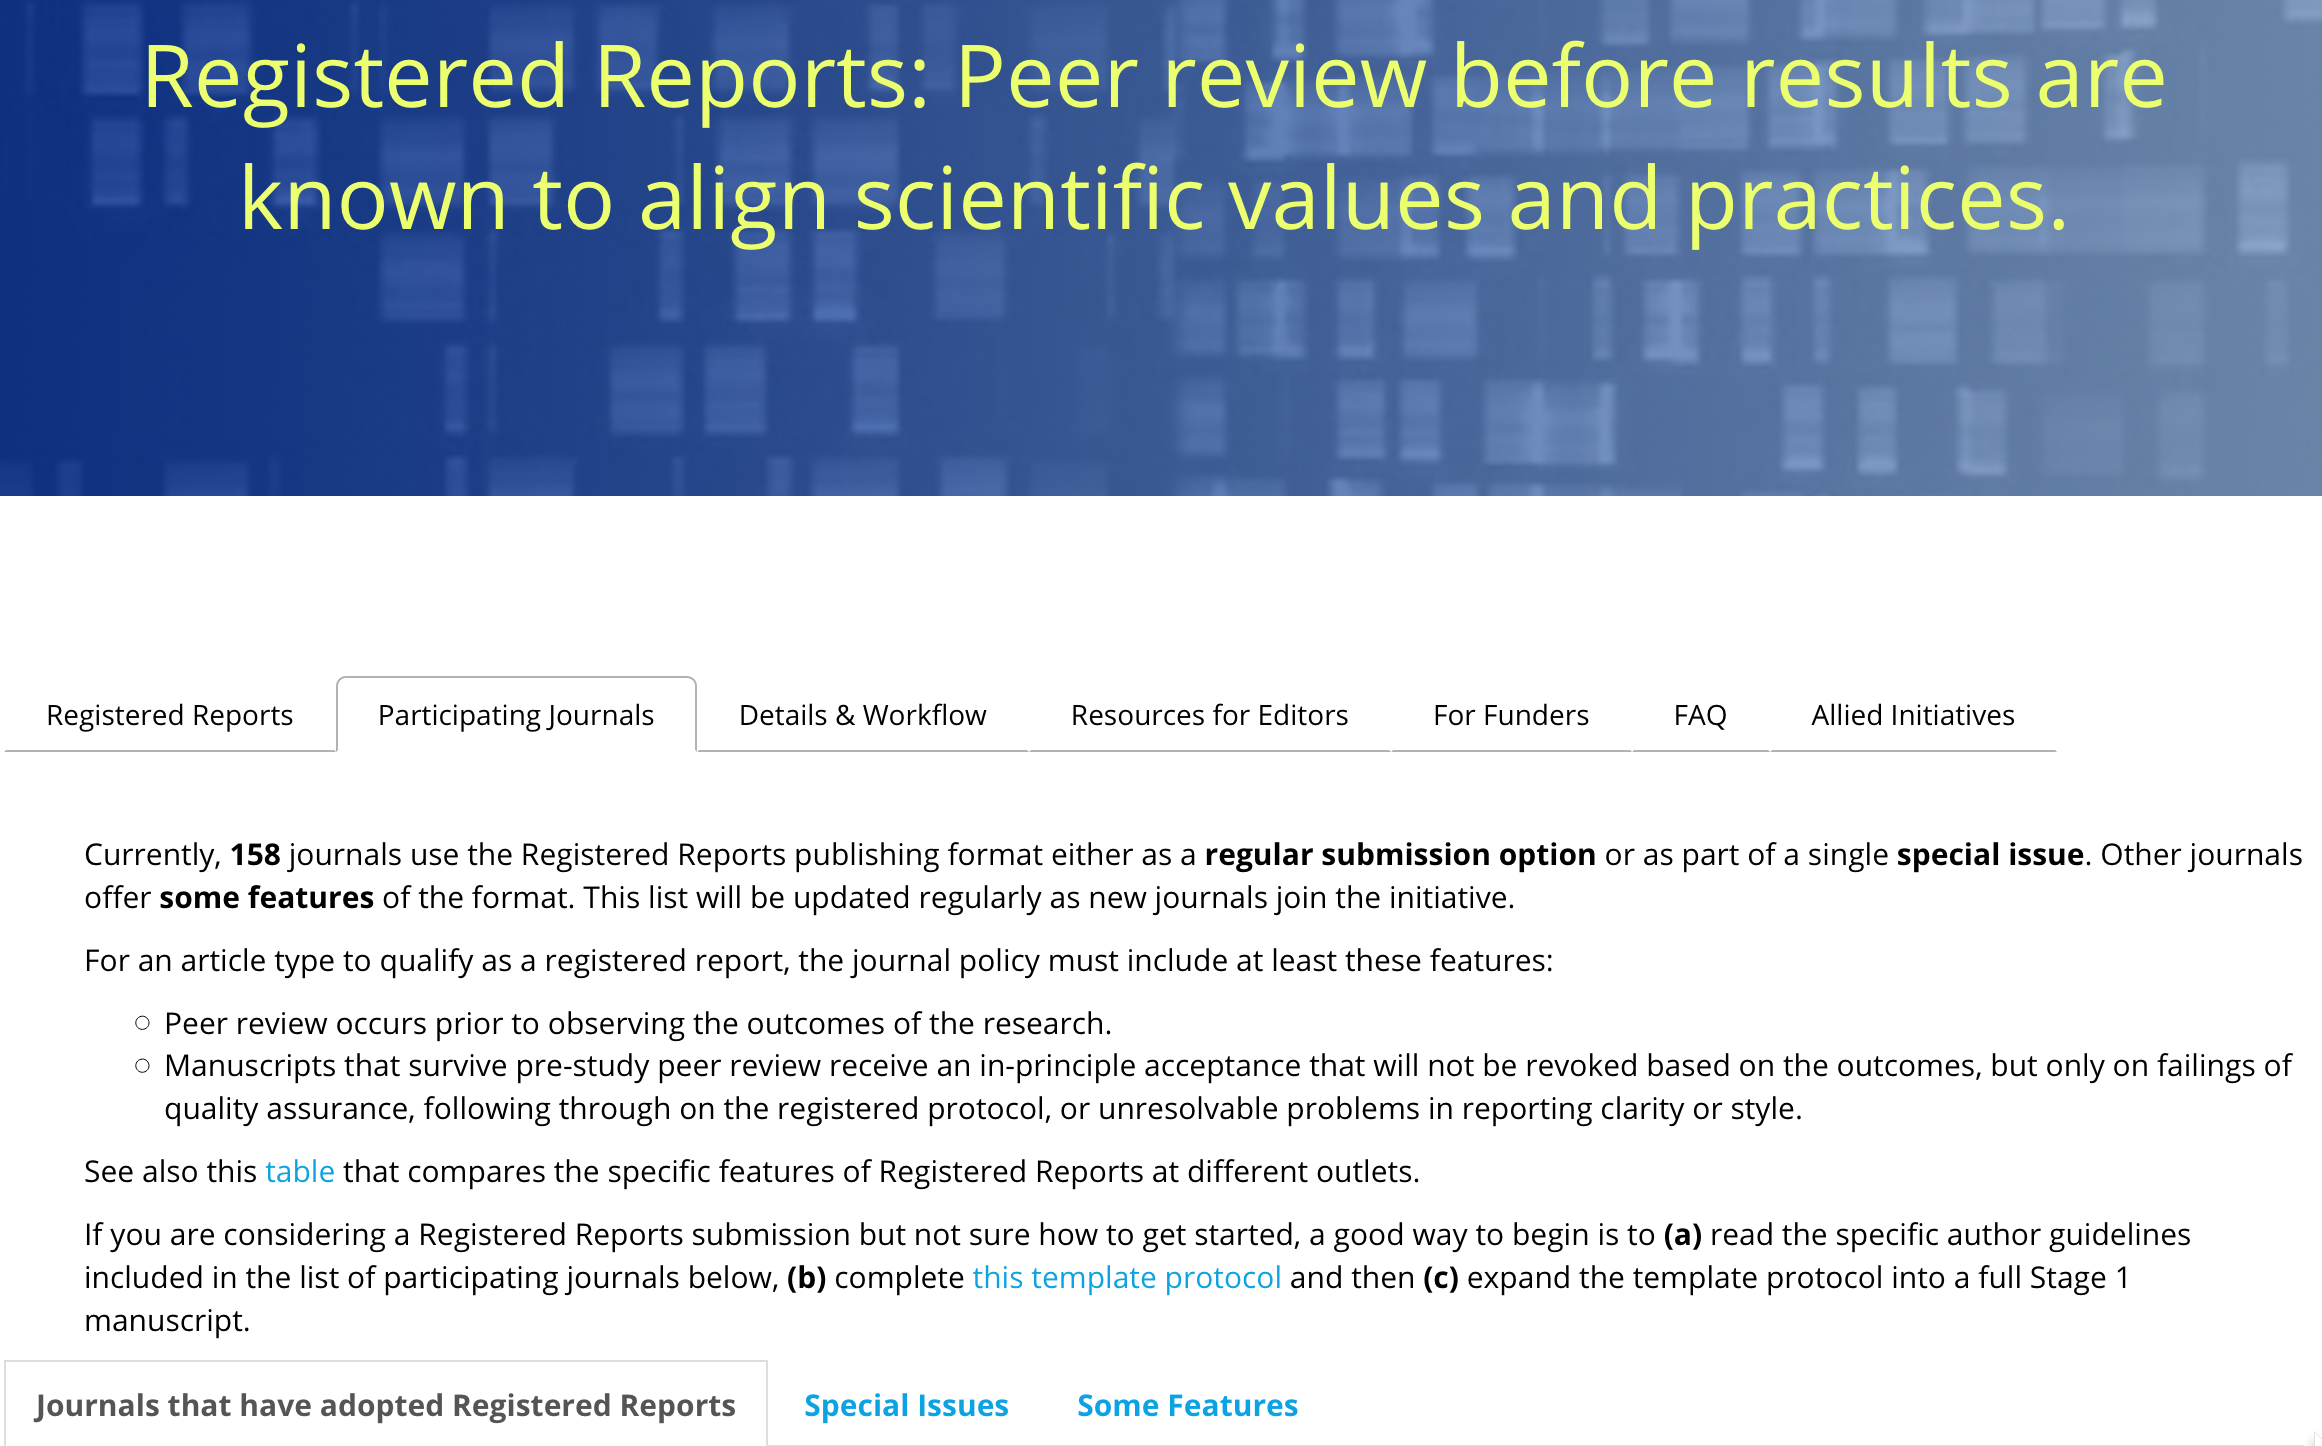
\includegraphics[scale=0.25]{rr.png}
\end{center}


\end{frame}


%------------------------------------------------

\begin{frame}
\frametitle{A solution: Share data and code}

 %\textbf{The sin of data hoarding}. \\[12pt]

Benefits of \textbf{sharing data and code}:
 
 \begin{itemize}
 \item independent researchers can repeat analyses 
 $\rightarrow$ helps to correct honest mistakes; ensures robustness of scientific record
 \item sharing materials also makes direct replication attempts easier \pause
 \item avoids (actual) responses like the following:
 \end{itemize}
 
 
\end{frame}

\begin{frame}
\frametitle{A solution: Share data and code}

 \begin{itemize}
 \item
 ``We have looked both in \dots and \dots, but I am sorry to say we can’t find those data anymore.''  \pause
 \item 
 ``\dots had to do some digging and finally found this file. I don’t know if that’s the ultimate version we used in the experiment, but it should be close. No idea about the fillers though. And I haven’t found the original data yet.'' \pause
 \item 
 ``Regarding the \dots data, \dots is the one who has it.  I have asked her a couple of times to send it, but she hasn't.  I think the data are at her parents home in \dots, but she doesn't go there often, because I don't think she gets along so well with her family.  I will ask her again for the data, but I don't know how long it will take for her to send it.''  \pause
 \item 
 ``I'm happy to provide our data for your project. During the summer, I don't visit my office regularly and that is where those data are stored, so it might be a few weeks before I send it along.''
 \end{itemize}
\end{frame}

%------------------------------------------------

\begin{frame}
\frametitle{Good practice}

 \textbf{``The sin of data hoarding''}\\[12pt]
 
 Major journals require authors to retain data for several years and share it with reader on request.
In 2006, Jelte Wicherts and colleagues tested this by requesting data from 249 studies that appeared in four major journals.\\[12pt]
 
 
 ``Unfortunately, 6 months later, after writing more than 400 emails---and sending some corresponding authors detailed descriptions of our study aims, (...)---we ended up with a meagre 38 positive reactions and the actual data sets from 64 studies (26\% of the total number of 249 data sets).''
 
 \begin{itemize}
 \item 18\% did not respond
 \item 35\% refused to share data
 \item 20\% promised to send it but never did
 \item all studies had been published in the previous 18 months
  \end{itemize}
  
 \end{frame}

%------------------------------------------------

\begin{frame}
\frametitle{Further reading}
% many other advantages to pre-registrating studies prior to data collection. 

\begin{center}

\includegraphics[scale=0.2]{chambers.png}
\end{center}

\begin{footnotesize}
Chambers, C. (2017). The Seven Deadly Sins of Psychology. Princeton University Press. 
\end{footnotesize}

\end{frame}

%-----------------------------------------------


\begin{frame}

\frametitle{Pre-Registration}

\begin{large}

\textbf{Potential problem with registered reports}

\begin{itemize}
\item  Loss of time because (a) paper has to be written, (b) have to wait for reviews, (c) have to respond to reviews, even before collecting any data. 
\end{itemize}

\textbf{Solution: Pre-registration without peer review}
\begin{itemize}
\item E.g. on Open Science Framework (\url{https://osf.io/}), or 
\item AsPredicted (\url{https://aspredicted.org/}) \\[30pt]
\end{itemize}


\end{large}

\begin{tiny}
Source: Chambers, C. (2017). The Seven Deadly Sins of Psychology. Princeton University Press. 
\end{tiny}
\end{frame}

%-----------------------------------------------
\begin{frame}
\frametitle{Registered Reports}

\begin{center}
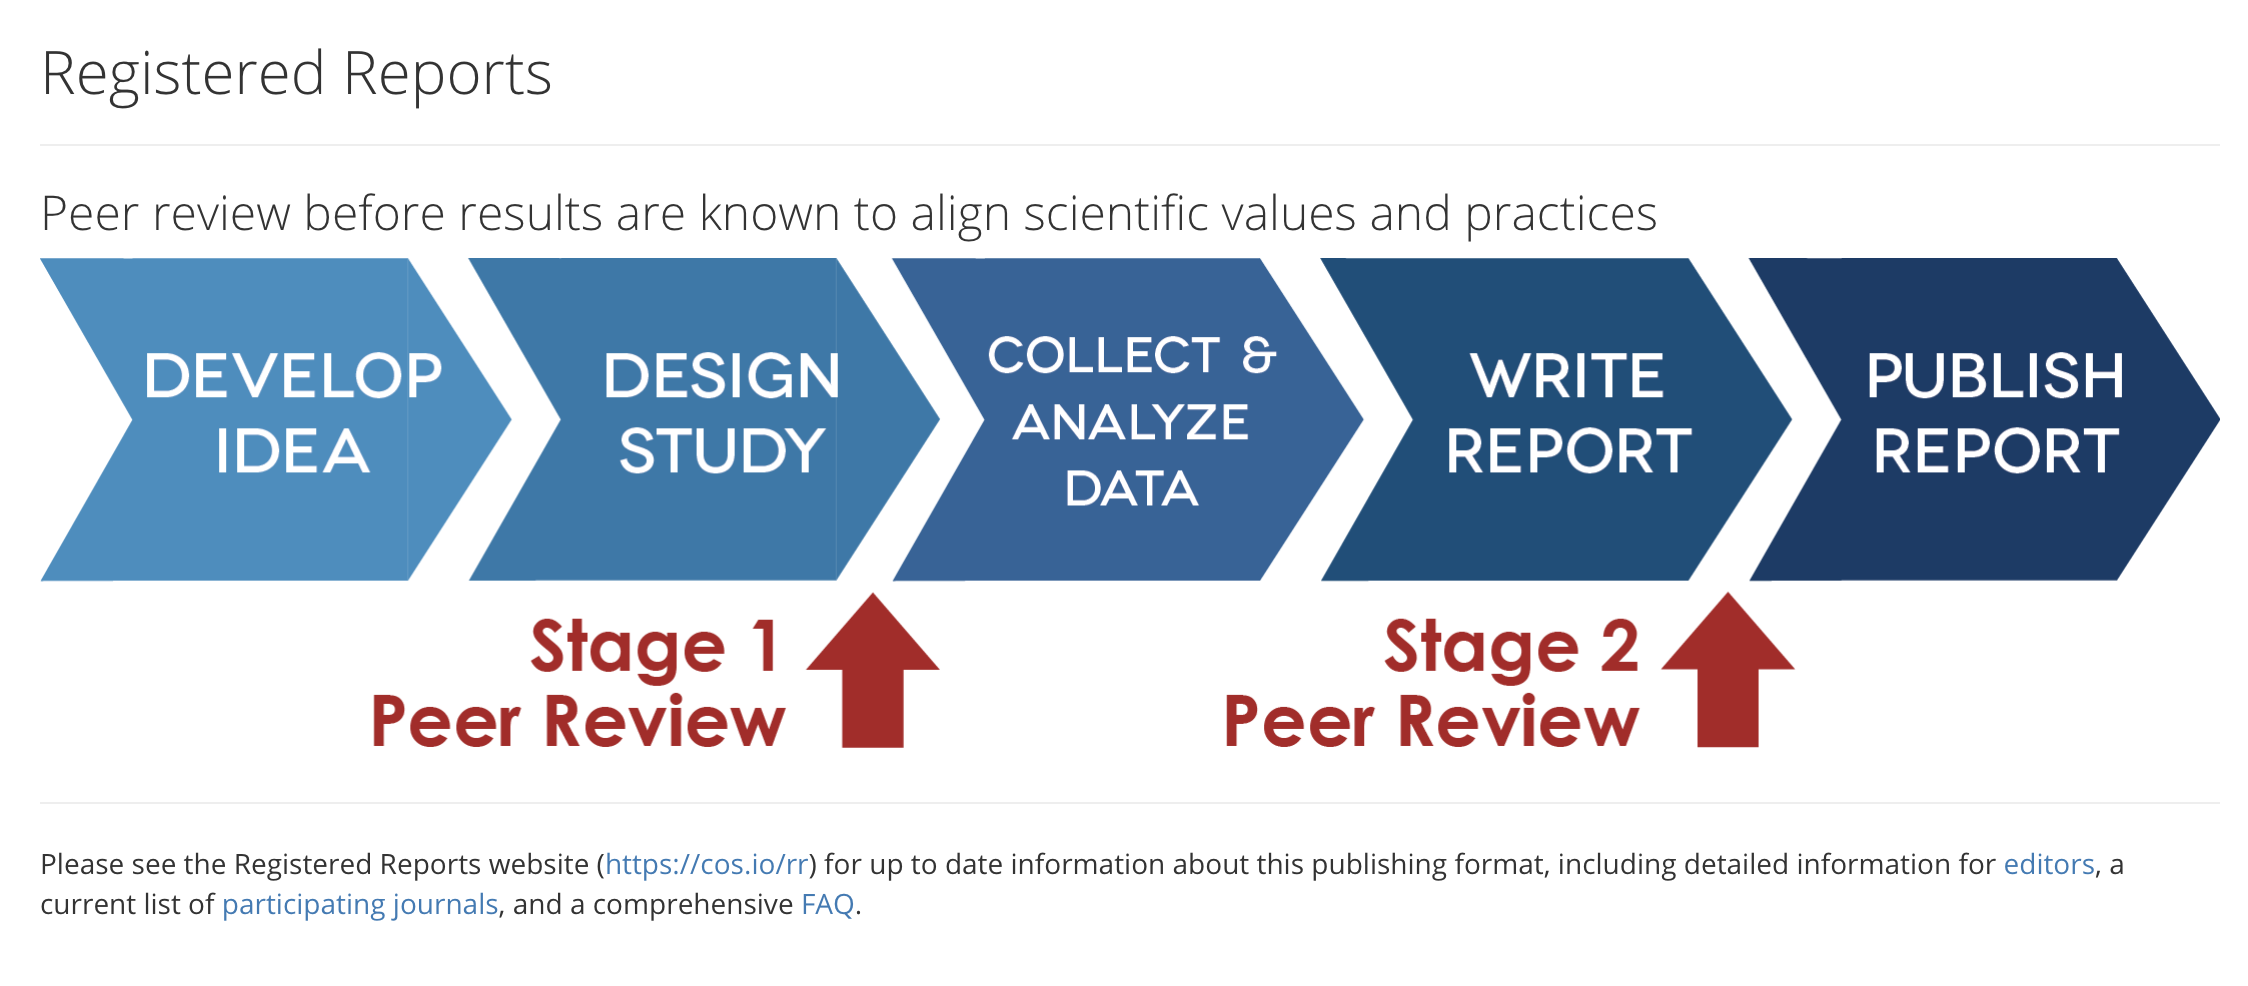
\includegraphics[scale=0.23]{RegRep.png}
\end{center}


\begin{large}
\textbf{Stage 1}
\begin{itemize}
\item<1-> Manuscript (incl. hypotheses, methods, planned analyses) is submitted.
\item<2-> Stage 1 peer review (incl.\ `Does the proposed study have sufficient power?') 
\item<3> `In Principle Acceptance' \textit{independent of results}. 
\end{itemize}

\end{large}




\begin{tiny}
Source: https://osf.io/8mpji/wiki/home/
\end{tiny}
\end{frame}

%-----------------------------------------------
\begin{frame}
\frametitle{Registered Reports}

\begin{large}


\textbf{Stage 2}
\begin{itemize}
 \item Study is conducted. 
\pause \item Manuscript is resubmitted (+ results, discussion).
\begin{itemize}
\begin{large}
\pause \item results: confirmatory \textbf{and} exploratory analyses.
\end{large}
\end{itemize}
\pause \item Stage 2 peer review. %did authors follow approved protocol? do the data justify the conclusions?
\pause \item Publication of manuscript. \\[20pt]
\end{itemize}



For detailed authors' guidelines see \href{http://bit.ly/cortexinstructions}{\textcolor{blue}{http://bit.ly/cortexinstructions}}.
\end{large}

\end{frame}



\begin{frame}
\frametitle{But \dots}

\textsc{...registered reports prevent exploration of data and curb scientific creativity.}\\[12pt]

\pause

\textbf{Verdict: False.} Authors should feel free to perform unregistered exploratory analyses with as much creativity as they can muster, the only requirement is that such analyses are labeled as exploratory. 


\end{frame}
%-----------------------------------------------
\begin{frame}
\frametitle{But \dots}

\textsc{...Registered reports are not suitable for exploratory science or for developing new methods where there are no hypotheses.}\\[12pt]

\pause

\textbf{Verdict: Red herring.} Irrelevant objection. Format not designed to be applicable to anything other than hypothesis-driven science.  

\end{frame}

%-----------------------------------------------

\begin{frame}
\frametitle{But \dots}

\textsc{...registered reports can be gamed by ``preregistering'' a study that is already completed.}\\[12pt]

\pause

\textbf{Verdict: True only for fraudsters.}  

\end{frame}

%-----------------------------------------------


\begin{frame}
\frametitle{But \dots}

\textsc{Reviewers of Stage 1 submissions could steal my ideas and scoop me.}\\[12pt]
\pause

\textbf{Verdict: Possible but highly unlikely.} Concern does not stop researchers from applying for grant funding or presenting ideas at conferences $\rightarrow$ much larger group of potential competitors.\\
Also, once in-principle acceptance awarded, journal cannot reject Stage 2 submission, because similar work was published elsewhere.  
\end{frame}

%-----------------------------------------------


\begin{frame}
\frametitle{But \dots}

\textsc{...registered reports lock authors into publishing with a specific journal.}\\[12pt]

\pause

\textbf{Verdict: False.} Withdrawal of registered report is possible at any time. After in-principle acceptance: publication of withdrawn registration (includes abstract from Stage 1 submission and reason for withdrawal). Ensures process is transparent to scientific community. 

\end{frame}

%-----------------------------------------------



\begin{frame}
\frametitle{But \dots}

\textsc{...We don't need registered reports because we have replication.}\\[12pt]

\pause

\textbf{Verdict: False.} Argument ignores the fact that direct replication in psychology is extremely rare; associated with disincentives, such as journals' want for novelty. \\Pre-registration could have positive impact: provisional acceptance of papers before investing resources. 
\end{frame}
% direct vs conceptual replication: conceptual: similar design, but we add something novel to the study, change method, so its publishable: these can confirm but never refute previous findings 

%-----------------------------------------------

\begin{frame}
\frametitle{But \dots}

\textsc{...The case for Registered Reports assumes that scientists act dishonestly, and sends the message that there is no trust in the scientific community.}\\[12pt]

\pause

\textbf{Verdict: Red herring.}
Argument rests on false premise that bad practice is synonymous with deliberate deceit.\\ Bias and questionable research practices can be unconscious or stem from ignorance without implying any dishonesty.\\ Argument places greater emphasis on how we feel than on how research is actually conducted. \\
Regardless of conscious or unconscious ``bad practice'', the solutions are the same. 
\end{frame}




%-----------------------------------------------

\begin{frame}
\frametitle{Pre-registration at OSF -- What has to be done?}
\begin{enumerate}
\item Registration at \url{https://osf.io/}.
\item Creation of a project.
\item Insertion of an abstract for the project:
\end{enumerate}
\begin{center}

\includegraphics[scale=0.4]{prereg1.pdf}
\end{center}
\end{frame}
%------------------------------------------------
%------------------------------------------------

\begin{frame}
\frametitle{Upload the project}
\begin{itemize}
		\item[a] Upload the whole project as one PDF file.
		\item[] alternatively:
		\item[b] Upload the components of the project.
\end{itemize}
\end{frame}
%------------------------------------------------
%------------------------------------------------

\begin{frame}
\frametitle{Upload the project}
\begin{itemize}
		\item[a] Upload the whole project as one PDF file
		\item Inclusion of:
		\begin{itemize}
			\item aim of the study, 
			\item hypotheses \& predictions, 
			\item procedure, 
			\item design (including example item), 
			\item stopping rule,
			\item analysis plan
		\end{itemize}
\end{itemize}
\end{frame}
%------------------------------------------------
%------------------------------------------------

\begin{frame}
\frametitle{Upload the project}
\begin{itemize}
		\item[b] Upload the components of the project:
\end{itemize}
\begin{center}
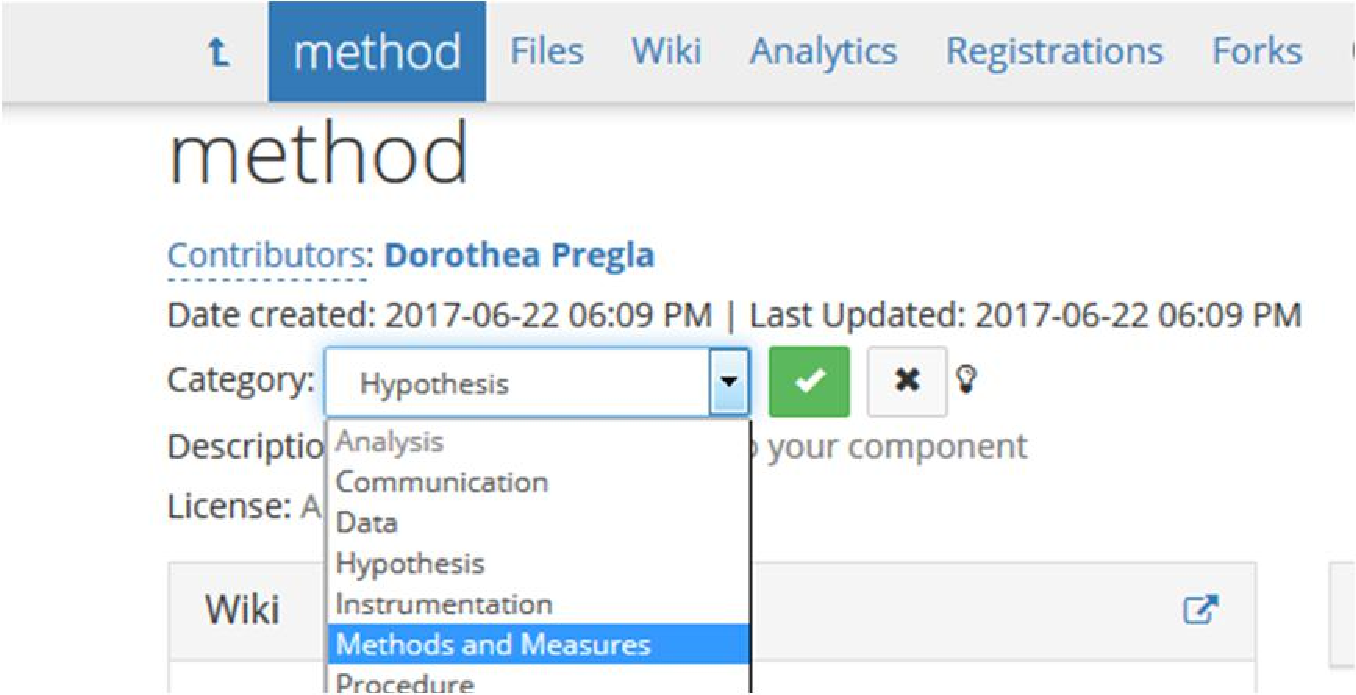
\includegraphics[scale=0.4]{prereg2.pdf}
\end{center}
\end{frame}
%------------------------------------------------
%------------------------------------------------

\begin{frame}
\frametitle{Who can see the project?}
\begin{itemize}
	\item Certain parts or the whole project can be \textit{made public}.
	\item The project is not visible to anyone as long as it is not made public.
	\item To make the project public select those parts that shall be public:
\end{itemize}
\begin{center}
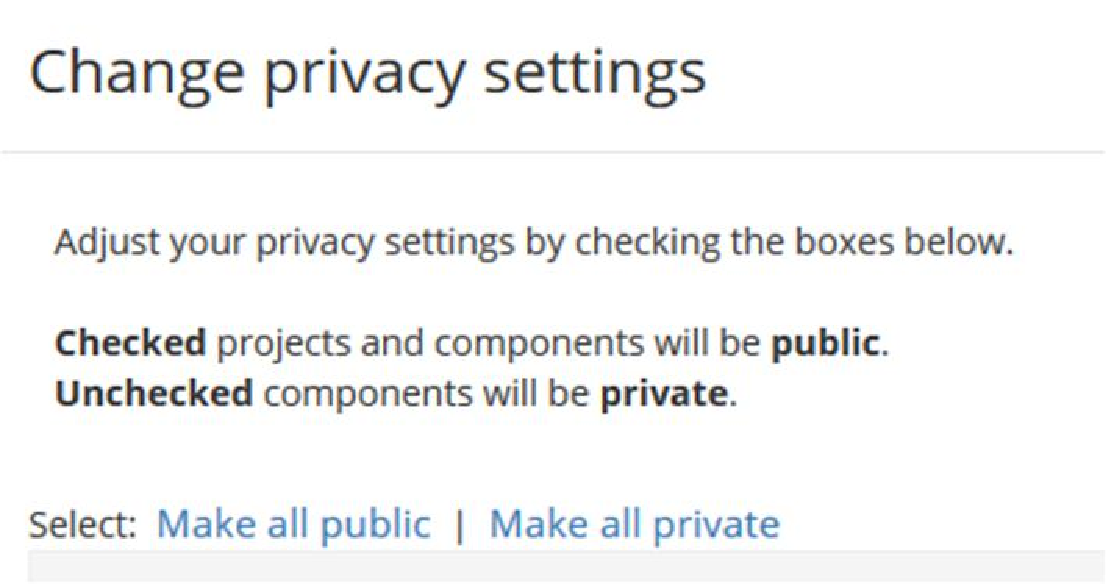
\includegraphics[scale=0.4]{prereg3.pdf}
\end{center}
\end{frame}
%------------------------------------------------
%------------------------------------------------

\begin{frame}
\frametitle{Who can see the project?}
\begin{itemize}
	\item Public parts can be seen by anyone \\ (including unregistered visitors of OSF).
	\item Public parts can be made private again.
 	\item Projects can be pre-registered without making them public.
\end{itemize}

\end{frame}
%------------------------------------------------
%------------------------------------------------

\begin{frame}
\frametitle{How to pre-register a project}
\begin{itemize}
	\item[1] Select a registration method (e.g. OSF-Standard)
\end{itemize}
\begin{center}
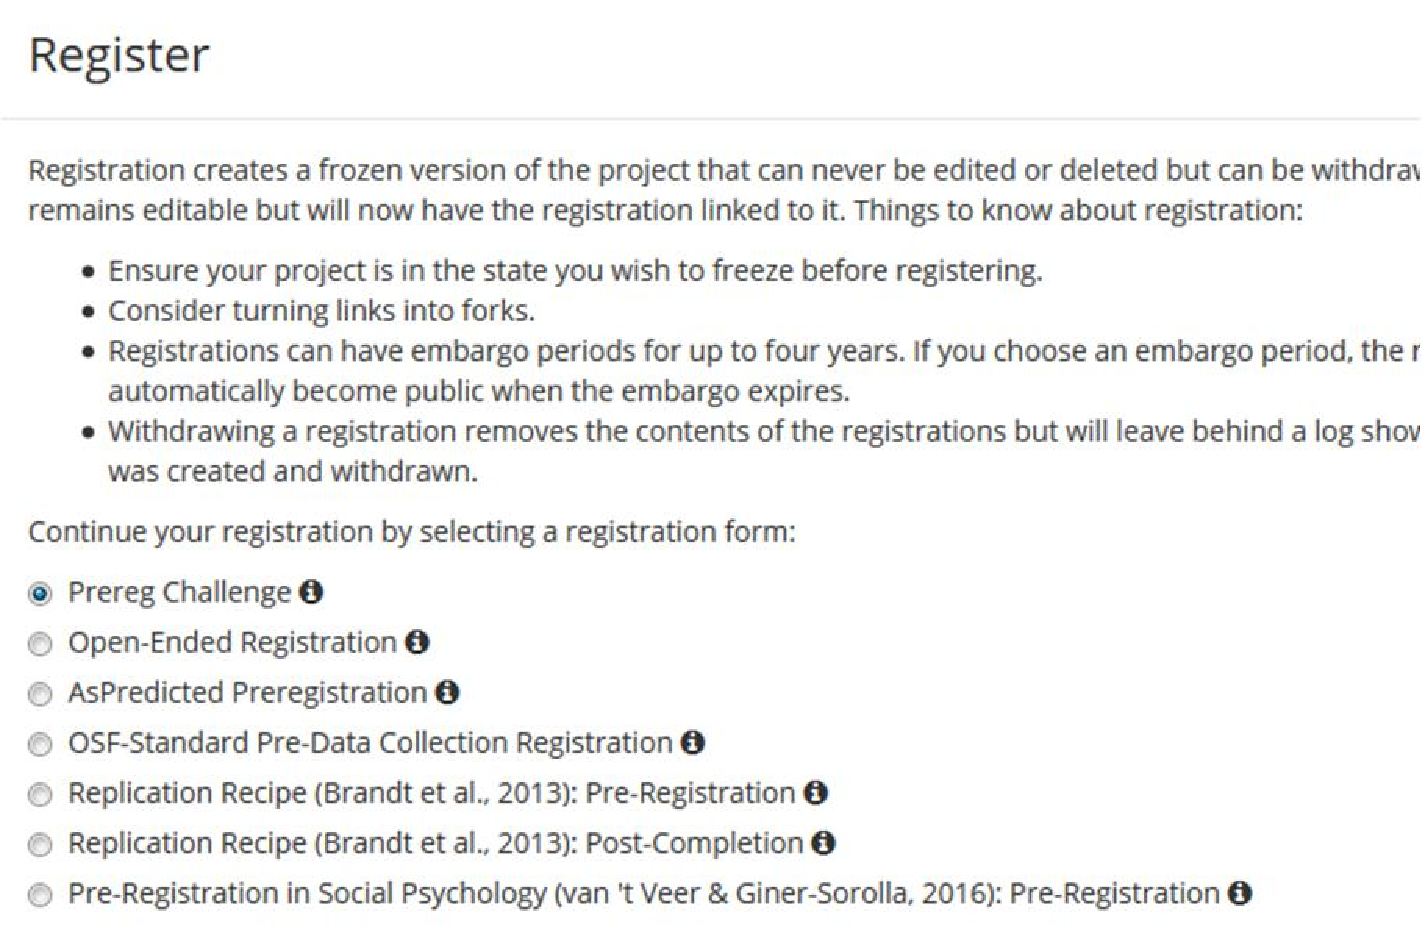
\includegraphics[scale=0.4]{prereg4.pdf}
\end{center}
\end{frame}
%------------------------------------------------
%------------------------------------------------

\begin{frame}
\frametitle{How to pre-register a project}
\begin{itemize}
	\item[2] Fill in the registration form \& submit it.
\end{itemize}
\begin{center}
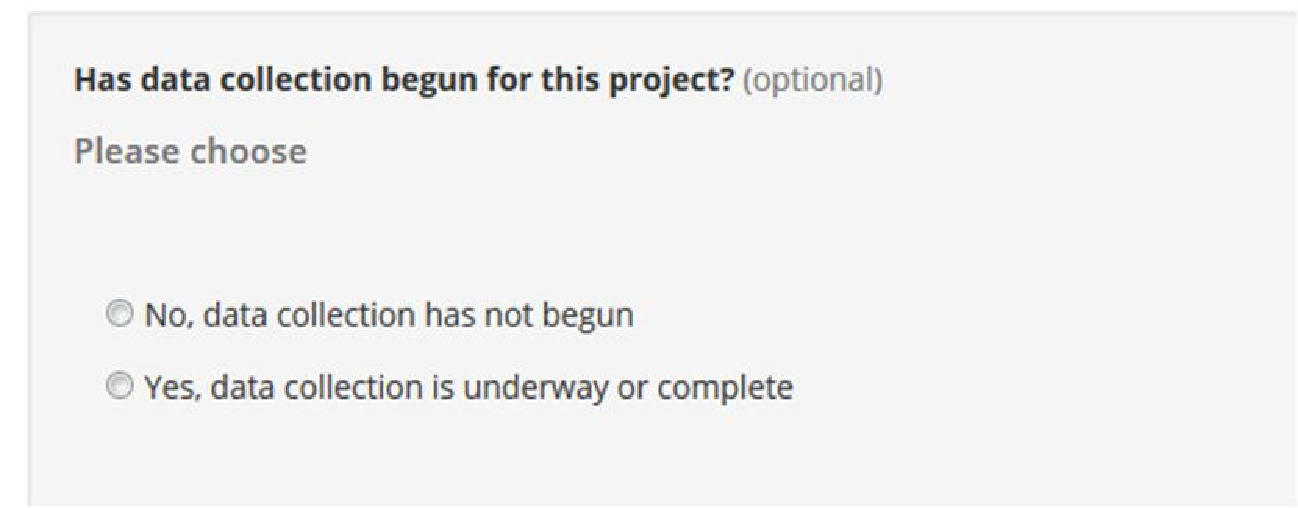
\includegraphics[scale=0.4]{prereg5.pdf}
\end{center}
\begin{itemize}
	\item[3] Link the pre-registration when the study is submitted for publication.
\end{itemize}
\end{frame}
%------------------------------------------------
\begin{frame}
\frametitle{How to pre-register a project}

\begin{LARGE}


Find the OSF pre-registration instructions here:

\url{http://bit.ly/Q_SFB1287}

\end{LARGE}

\end{frame}
%------------------------------------------------

\begin{frame}
\frametitle{What has changed for my lab after adopting these practices?}

\begin{itemize}
\item Slower data collection and publication: 
\begin{itemize}
\item 7 papers in 2018
\item 6 in 2017
\item 11 in 2016
\item  10 in 2015
\end{itemize}
\item  Discuss the ambiguities of the results openly in papers. 
\item Occasionally got rejected from a top journal because ``story didn't bring closure.''
\item Releasing data caught mistakes before publication.
\end{itemize}

Overall, I feel that the quality of our work has improved. 

\end{frame}


\end{document} 

